\documentclass{beamer}

\usepackage[T1]{fontenc}
\usepackage[utf8]{inputenc}
\usepackage[ngerman]{babel}
\usepackage{default}
\usepackage{amsmath}
\usepackage{amssymb}
\usepackage{graphicx}
\usepackage{transparent} %more transparent images
\usepackage{textcomp}
\usepackage{multimedia}%um Filme einzubinden
\usepackage{verbatim}%für comment
%\usepackage{wrapfig}%umfliesse einer grafik mit text
\usepackage{caption} %für Subfigure
%\usepackage{subcaption} %für Subfigure
\usepackage{wrapfig} %für wrapfigure umgebungen, eigentlich für fließbilder, klappt bei mir aber net
\usetheme{Warsaw}
\usecolortheme{seahorse}
%\useinnertheme{circles}
%\useoutertheme{tree}
\usepackage{tikz} %fuer baumdiagramme. mehr unter:
\usetikzlibrary{calc, shapes, backgrounds} %http://www.texample.net/tikz/examples/coin-flipping/
\usetikzlibrary{automata,arrows,decorations.pathmorphing,backgrounds,positioning,fit,petri}  %fuer das zeichnen von automaten. steht unter gelichem link seite 42
\usepackage{subfigure}
%C++
\usepackage{listings}
\usepackage{color}
%
%
\usepackage{lmodern} %for distance between some items 


\useoutertheme{infolines}
\usepackage{hyperref}

%siehe für folgendes: 
%http://tex.stackexchange.com/questions/56860/how-to-modify-outer-theme-infolines-to-include-the-title-and-section-in-the-head

\setbeamertemplate{headline}
{  \leavevmode%
  \hbox{%
  \begin{beamercolorbox}[wd=.5\paperwidth,ht=4.25ex,dp=1ex,right,rightskip=1em]{section in head/foot}%
    \usebeamerfont{subsection in head/foot}\hspace*{2ex} \large{\insertsectionhead} %\hspace*{1ex}%\vspace{0.05em}
  \end{beamercolorbox}%
  \begin{beamercolorbox}[wd=.5\paperwidth,ht=4.25ex,dp=1ex,left,leftskip=1em]{subsection in head/foot}%
    \usebeamerfont{section in head/foot}\large{\insertsubsectionhead} %\vspace{0.1em}
  \end{beamercolorbox}%
   } 
  \vskip2pt%
}

\setbeamertemplate{footline}
{
  \leavevmode%
  \hbox{%
  \begin{beamercolorbox}[wd=.5\paperwidth,ht=2.25ex,dp=1ex,left,leftskip=1em]{author in head/foot}
  % statt left auch die Orientierung center oder right
    \usebeamerfont{author in head/foot}\insertshortauthor%~~\beamer@ifempty{\insertshortinstitute}{}{(\insertshortinstitute)}
  \end{beamercolorbox}%
  \begin{beamercolorbox}[wd=.5\paperwidth,ht=2.25ex,dp=1ex,right]{date in head/foot}%
    \usebeamerfont{date in head/foot}\insertshortdate{}\hspace*{2em}
    \insertframenumber{} / \inserttotalframenumber\hspace*{2ex} 
  \end{beamercolorbox}}%
  \vskip0pt%
}



\setbeamertemplate
    {frametitle}
    {
    \leavevmode
    \begin{beamercolorbox}[wd=1\paperwidth,ht=4.25ex,dp=2ex,center]{author in head/foot}
     
       \Huge \insertframetitle
   
      \end{beamercolorbox}
      \vskip0pt%
    }
\setbeamertemplate{navigation symbols}{}
%\setbeamertemplate{section in toc}[sections numbered]
%\setbeamertemplate{subsection in toc}[subsections numbered]
%\setbeamerfont{frametitle}{size=\Huge}


%für C++ Quellcode
\definecolor{listinggray}{gray}{0.9}
\definecolor{lbcolor}{rgb}{0.9,0.9,0.9}
\lstset{
columns=fullflexible, %this is for copy pastable without whitespace
backgroundcolor=\color{lbcolor},
    tabsize=4,    
%   rulecolor=,
    language=C++,
        basicstyle=\scriptsize,
        upquote=true,
        aboveskip={1.5\baselineskip},
        columns=fixed,
        showstringspaces=false,
        extendedchars=false,
        breaklines=true,
        prebreak = \raisebox{0ex}[0ex][0ex]{\ensuremath{\hookleftarrow}},
        frame=single,
        numbers=left,
        showtabs=false,
        showspaces=false,
        showstringspaces=false,
        identifierstyle=\ttfamily,
        keywordstyle=\color[rgb]{0,0,1},
        commentstyle=\color[rgb]{0.5,0.05,0.05},%{0.026,0.112,0.095},
        stringstyle=\color[rgb]{0.627,0.126,0.941},
        numberstyle=\color[rgb]{0.205, 0.142, 0.73},
	emph={std,unique_ptr, string, move, ::},
	emphstyle={\color{blue}}
        %red=\color[rgb]{1,0,0}
        %Darkgreen=\color[rgb]{0,1,0}
%        \lstdefinestyle{C++}{language=C++,style=numbers}’.
}

%Global Background must be put in preamble
\usebackgroundtemplate%
{%
    %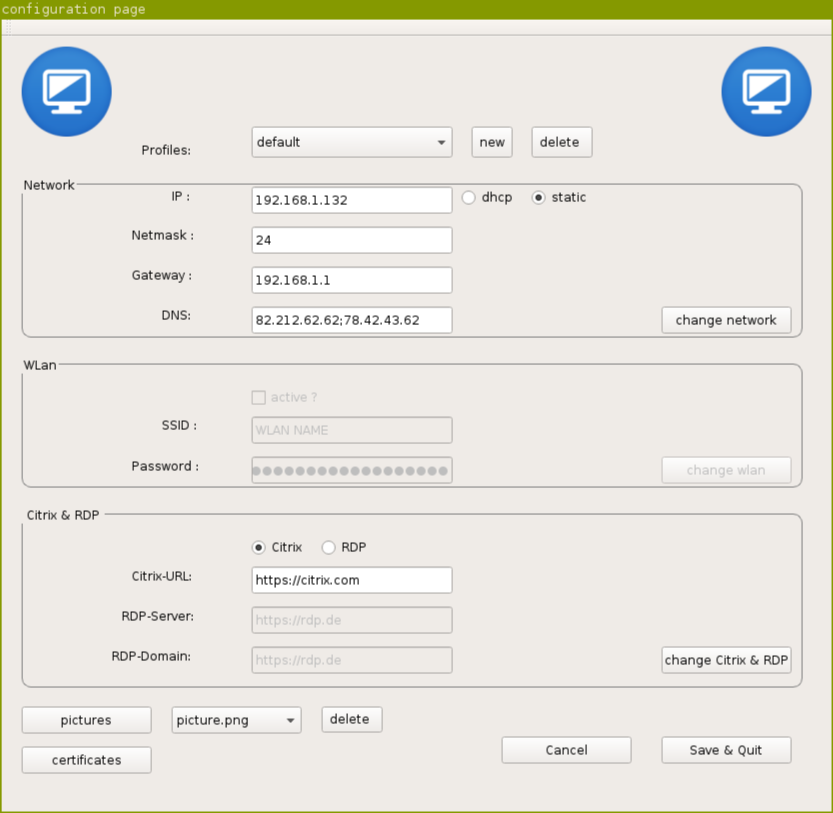
\includegraphics[width=\paperwidth,height=\paperheight]{ConfigPage}%
}


\title{Configuration Page}
%\subtitle{scientific working at the University of Heidelberg}
\institute{C++ Practice an der Universität Heidelberg}
\author{Cedrique Tassi \& Andreas Haller}
\date{26. Januar 2016}

\begin{document}
 %\huge



\maketitle

\begin{frame}
	\frametitle{Literatur}
	\centering
	Stroustrup, Bjarne: \textit{A Tour of C++}\\
	Upper Saddle River, NJ: Addison-Wesley, 2014\\
\vspace{2em}
	Unzählige Internetseiten\\
\end{frame}

\Large

\frame{
  \frametitle{Kapitel} 
  \begin{center}
		\begin{columns}
			\begin{column}{.35\linewidth}
				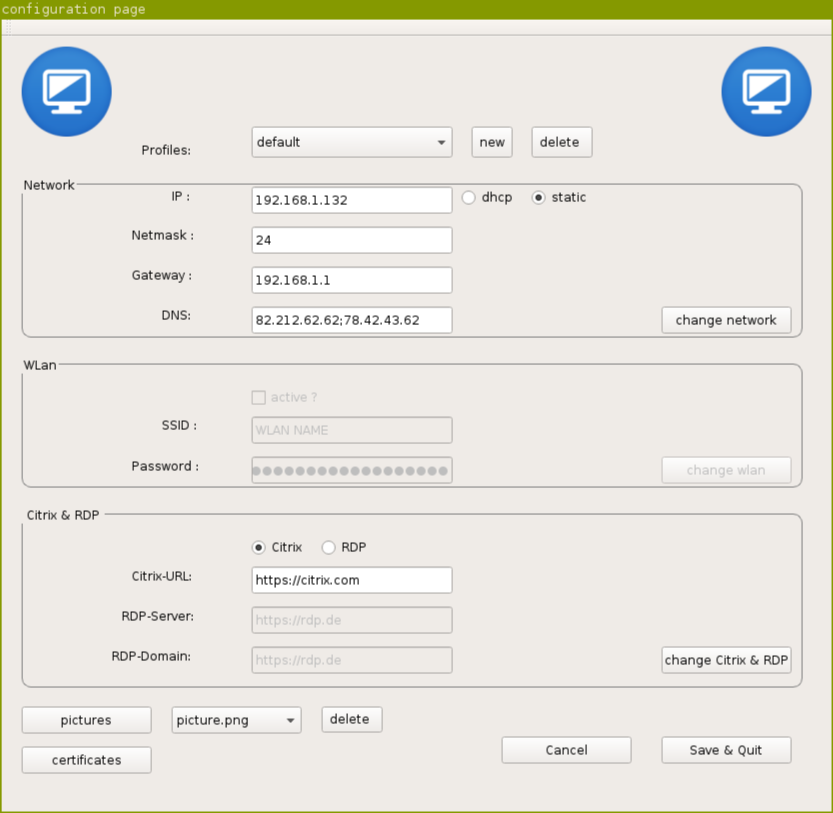
\includegraphics[scale=0.18]{ConfigPage}\\
			\end{column}
			\begin{column}{.65\linewidth}
				\tableofcontents%[pausesections] statt alles auf einmal mit Parameter nacheinander 
			\end{column}
		\end{columns}
  \end{center} 
}


%\raisebox{VERSCHIEBUNG}[HOEHER][TIEFE]{INHALT}


\section{Problemstellung}
	\begin{comment}
	Aufgrund der Mitarbeit von Andreas Haller bei dem Startup IT4S!?  stellte sich folgende Problemstellung:

	Es soll eine Verwaltungskonsole für ThinClients erstellt werden, 
	auf welcher man die Netzwerkeigenschaften konfigurieren kann, 
	damit eine Verbindung zum Server ermöglicht wird. 

	1. Was sind ThinClients?
	    Auf einem Server laufen virtuelle Maschinen. 
	    Um auf diese Maschinen zugreifen zu können, werden ThinClients als Frontend genutzt.   
	    In diesem Fall kommt die Kommmunikation über Citrix oder RDP zustande.

	2. Voraussetzungen & Motivation:
	    Es ist bereits eine Quick&Dirty Lösung von Andreas Haller in C mit GTK vorhanden gewesen. 
	    Diese war aufgrund der mangelnden GTK-Kenntnisse schwer optisch anzupassen und war sehr unzuverlässlich. 

	3. Erstellung Profile zur Speicherung von Benutzereinstellungen
	   Systemweite Konfigurationsdatei
	\end{comment}

%\tiny
\footnotesize
\subsection*{Anforderungen}
	\begin{frame}
		\begin{center}
			\begin{columns}
				\begin{column}{.60\linewidth}
					\centering
					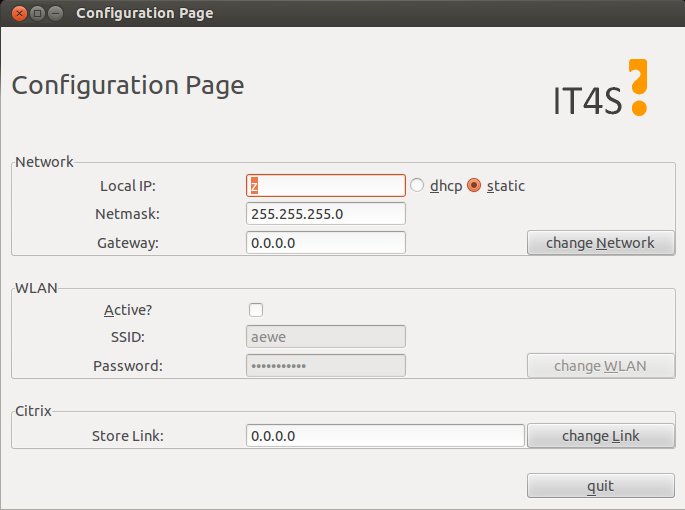
\includegraphics[scale=0.30]{gtk_oberflaeche}\\
				\end{column}
				\begin{column}{.4\linewidth}
					\vspace{5em}
					\begin{itemize}
						%3. Anforderungen an die Konfigurationsseite:
						%Folgende Punkte sollten manuell einstellbar sein.
						\item 	Benutzerprofile \& globale Einstellungen\\

						\item Netzwerktyp: dhcp/static\\
							IP, Netmask, Gateway, DNS 
							\vspace{1em}
						\item WLan aktiv/inaktiv, \\SSID, Passwort
							\vspace{1em}

						\item Verbindungstyp: Citrix/RDP\\
							Citrix-Link, RDP-Server, RDP-Domain

						\item Zertifikate \& Firmenlogo hinzufügen
					\end{itemize}
				\end{column}
			\end{columns}
		\end{center} 
	\end{frame}



\section{Konzept \& Realisierung}
	\begin{comment}
		Hier wird nun das Konzept der Umsetzung aus der Problemstellung vorgestellt. 
		Zuerst soll ein grober Zusammenhang dargestellt werden, wie alle Module miteinander zusammenhängen. 
		Danach wird expliziter auf die einzelnen Punkte eingegangen.

		Um eine bessere Vorstellung von der Konfigurationseite zu erhalten, ist hier die aktuelle Ansicht:
	\end{comment}
	\begin{frame}
		\centering
		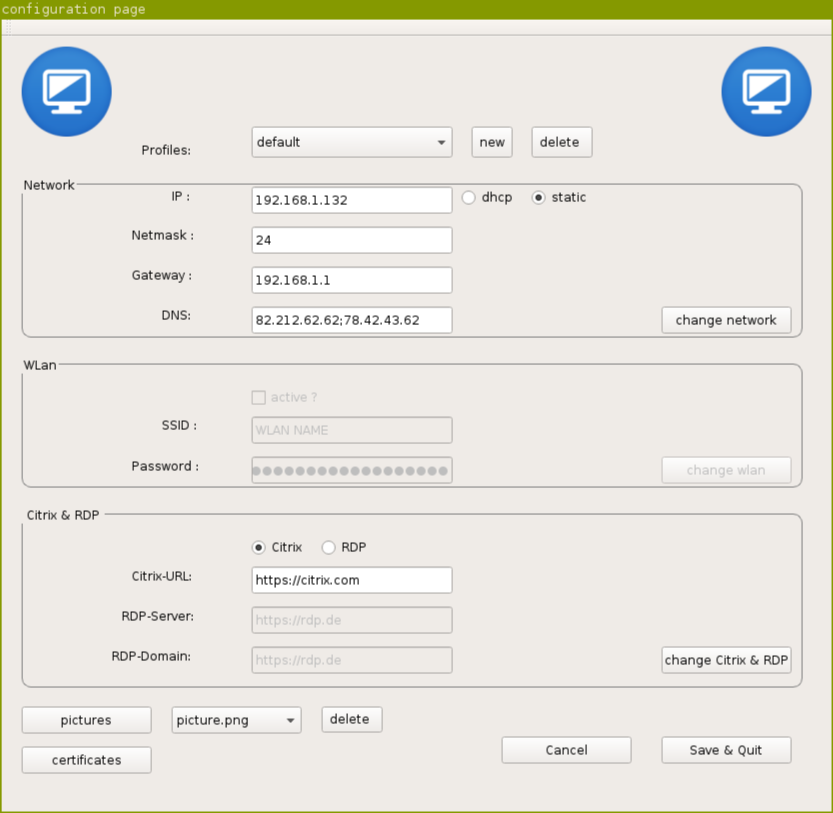
\includegraphics[scale=0.35]{ConfigPage}\\
			%\raisebox{-49mm}[5mm][5mm]{\includegraphics[scale=0.2]{../Bilder/spectrum}}
	\end{frame}


\subsection{Softwaremodulübersicht}
    \begin{frame}
		\centering
			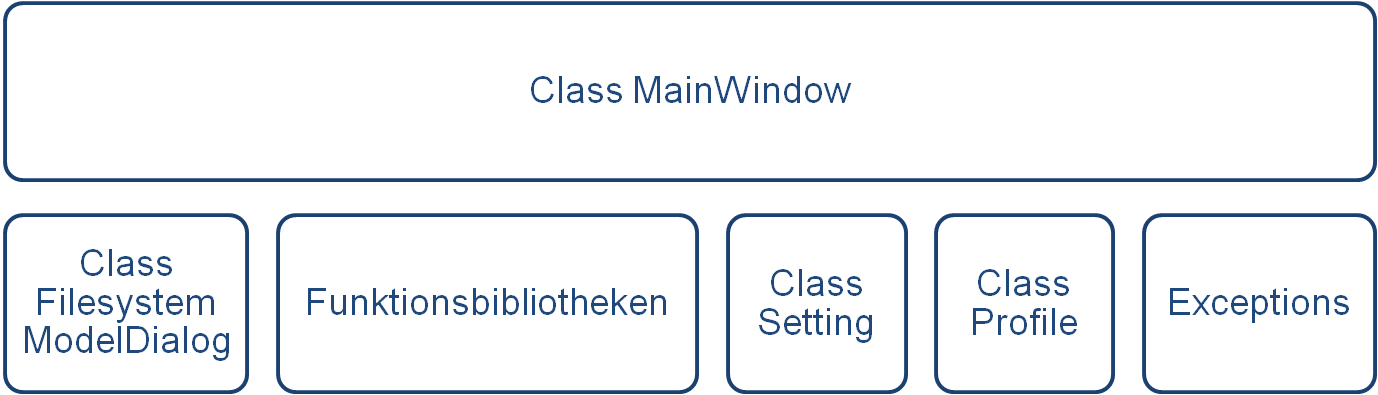
\includegraphics[width=\textwidth]{module.png}\\
			\vspace{3em}
			\Large Model View approach
	\end{frame}
	
\subsection{Implementierungsanforderungen}
	\begin{frame}
		\centering
		\begin{large}
			\begin{itemize}
				\item 	Aufbau von Qt-Klassen\\
                \vspace{1em}
				\item Erstellen von Dialogen\\
                \vspace{1em}
				\item SIGNAL und SLOT als Kommunikationsmechanismus\\
                \vspace{1em}
				\item Benutzen des Qt-Designers\\
                \vspace{1em}
				\item Robustheit und wiederverwendbarkeit
			\end{itemize}
		\end{large}
	\end{frame}
	
\subsection{Qt-Designer}
	\begin{frame}
		\centering
		\begin{large}
			\begin{itemize}
				\item 	Einfügen von GUI Komponenten per Drag\&Drop\\
                \vspace{1em}
				\item Setzen von Komponenteneigenschaften\\
                \vspace{1em}
				\item Verbinden von Signalen\\
                \vspace{1em}
				\item Erstellen des ui-Files   \\
			\end{itemize}
		\end{large}
		\vspace{3em}
		
\includegraphics[width=\textwidth]{designer.png}
	\end{frame}
	
\subsection{Setting \& Profile}
	\begin{frame}
		\centering
			\Large Die Klasse MainWindow\\
		    \vspace{1em}
			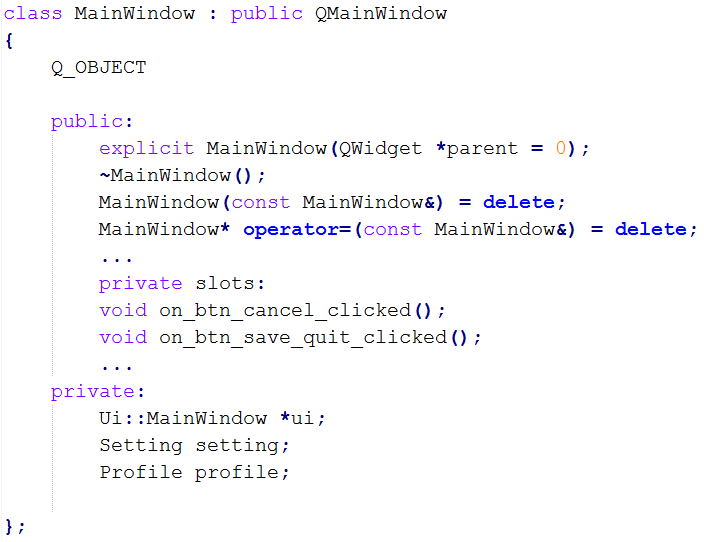
\includegraphics[width=0.8\textwidth]{main_window_code.png}\\
	\end{frame}
	
	\begin{frame}
		\centering
		\begin{large}
			\begin{itemize}
				\item 	Abgeleitet von QMainWindow\\
                \vspace{1em}
				\item Kapselt alle GUI-Komponenten \\(Qwidget, QGroupBox, QComboBox etc…)\\
                \vspace{1em}
				\item Enthält zwei Member-Objekten, Member-Funktionen und Slots\\
			\end{itemize}
			
		\end{large}
	\end{frame}
	
	\begin{frame}
		\centering
		    \Large Die Klasse Setting\\
		    \vspace{1em}
			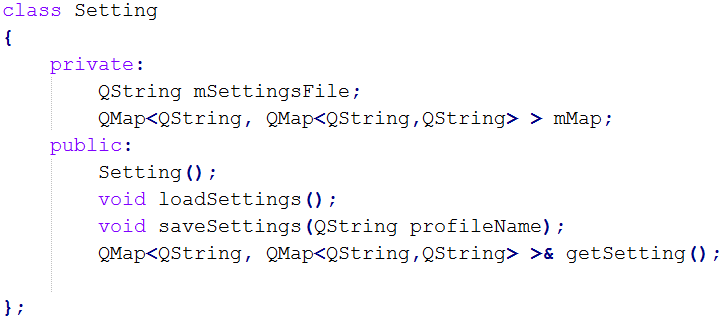
\includegraphics[width=0.8\textwidth]{string_code.png}\\
			\vspace{1em}
			\Large Der Member-Map dient zur Verwaltung der globalen Konfigurationsdatei
	\end{frame}

	\begin{frame}
		\centering
		\Large Globale Konfigurationsdatei (Setting.ini)\\
		\vspace{1em}
		\begin{large}
		    \frame{
            \begin{tabular}{|l|l|}
            \hline
            \textbf{keys} & \textbf{Values}  \\
            \hline
            path\_certificates & ../ConfigPage/certificates/  \\
            \hline
            path\_client\_logo &   ../ConfigPage/logo/client/\\
            \hline
            provider\_logo &  ../ConfigPage/logo/provider/ \\
            \hline
            path\_usb &  /media \\
            \hline
            path\_log & ../ConfigPage/log  \\
            \hline
            path\_profiles &  ../ConfigPage/profiles \\
            \hline
            last\_profile &  default \\
            \hline
            profile\_opt & current\_new  \\
            \hline
            system & arch, debian  \\
            \hline
             current\_client\_logo &   \\
            \hline
            \end{tabular}}
        	\end{large}
    \end{frame}
	
	\begin{frame}
		\centering
		    \Large Die Klasse Profile\\
		    \vspace{1em}
			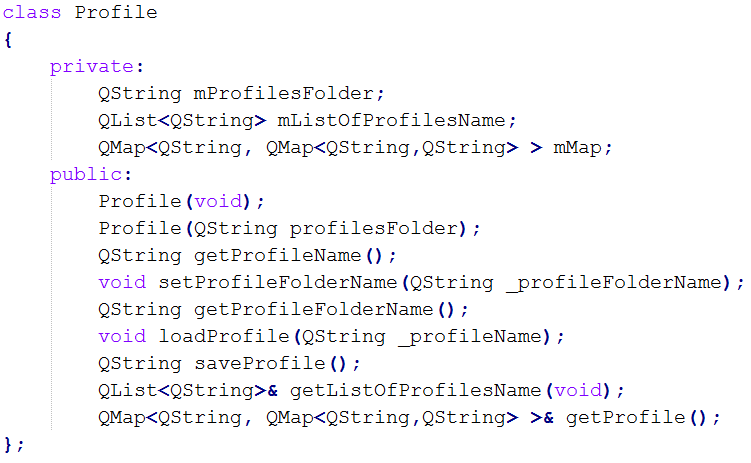
\includegraphics[width=\textwidth]{profile_code.png}\\
	\end{frame}
	
	\begin{frame}
		\centering
		\Large Aufbau einer Profile-Datei\\
		\vspace{1em}
		\begin{large}
		    \frame{
            \begin{tabular}{|l|l|}
            \hline
            \textbf{keys} & \textbf{Default-Values}  \\
            \hline
            citrix\_rdp\_citrix & https://citrix.com  \\
            \hline
            citrix\_rdp\_rdp\_domain &   https://rdp.de \\
            \hline
            citrix\_rdp\_rdp\_server &  https://rdp.de \\
            \hline
            citrix\_rdp\_type &  citrix \\
            \hline
            profile\_name & default  \\
            \hline
            network\_dns &  8.8.8.8 \\
            \hline
            network\_gateway &  192.10.100.1 \\
            \hline
            network\_netmask & 255.255.255.0  \\
            \hline
            network\_type & static  \\
            \hline
             wlan\_active &  true \\
            \hline
              \hline
             wlan\_passwd &  1234>? \\
            \hline
              \hline
             wlan\_ssid &  "WLAN; NA" \\
            \hline
            \end{tabular}}
        	\end{large}
\end{frame}

\subsection{Bilder \& Zertifikate}
	\begin{frame}
		\centering
		    \Large Auszug aus der Klasse FileSystemModelDialog\\
		    \vspace{1em}
			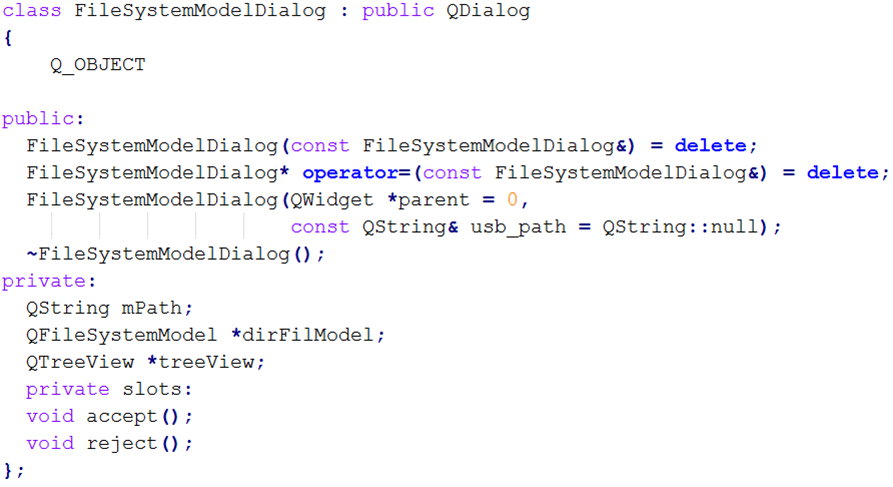
\includegraphics[width=0.8\textwidth]{filesystemModelDialog.png}\\
	\end{frame}
	
	\begin{frame}
		\centering
		\Large Warum FileSystemModelDialog anstatt QFileDialog ?\\
		\vspace{1em}
		\begin{large}
			\begin{itemize}
				\item QFileDialog ermöglicht stets das Navigieren durch komplettes Dateisystem, selbst beim Festlegen des RootPathDir\\
                \vspace{1em}
				\item Nur usb\_path sollte sichtbar sein\\
                \vspace{1em}
				\item ModelView mit QTreeView \& QDirModel\\
			\end{itemize}
			
		\end{large}
	\end{frame}
	
	\begin{frame}
		\centering
			\Large Flussdiagramm zum Hochladen von Bildern \& Zertifikaten\\
		    \vspace{1em}
			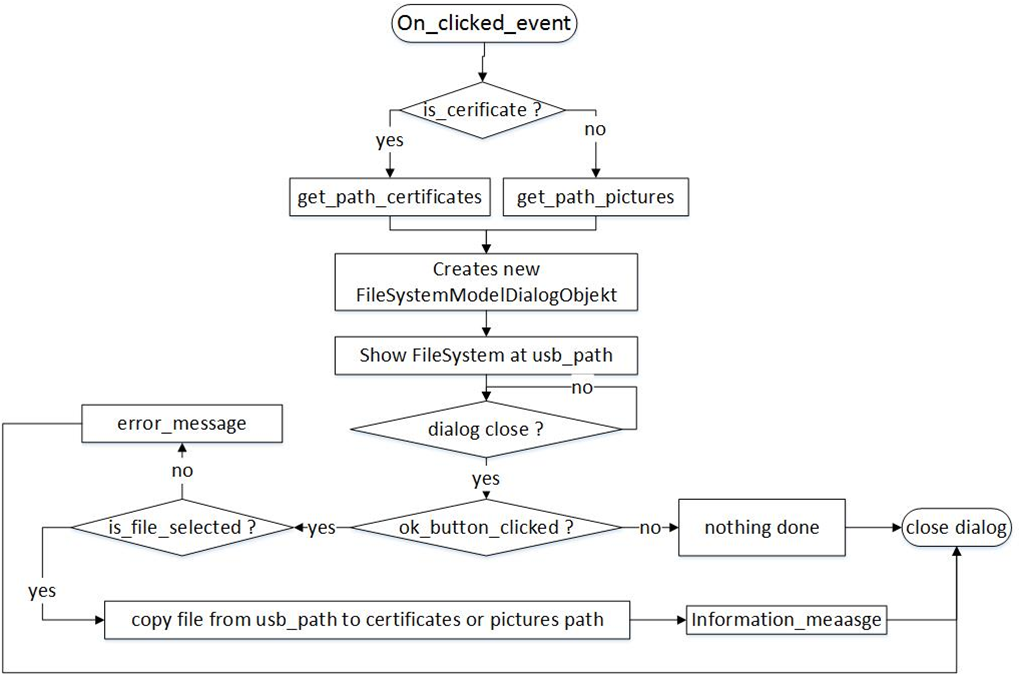
\includegraphics[width=0.8\textwidth]{flussdiagramm.png}\\
	\end{frame}


\subsection{Fehlerbehandlung}

\begin{comment}
%%%%%%%%%%%%%%%%%%%%%%%%%%%%%%%
%exception
%%%%%%%%%%%%%%%%%%%%%%%%%%%%%%%
\defverbatim[colored]\exception{
\begin{lstlisting}
class customer_error: public std::runtime_error{
	public:
	customer_error(std::string msg):runtime_error(msg){}
};
\end{lstlisting}
}
	\begin{frame}
\large
		\begin{center}
			\begin{columns}
				\begin{column}{.05\linewidth}
				\end{column}
				\begin{column}{.85\linewidth}
					\exception
				\end{column}
			\end{columns}
\Large




		\end{center} 
	\end{frame}

\end{comment}




% Local background must be enclosed by curly braces for grouping.
{
\usebackgroundtemplate{{\transparent{0.4}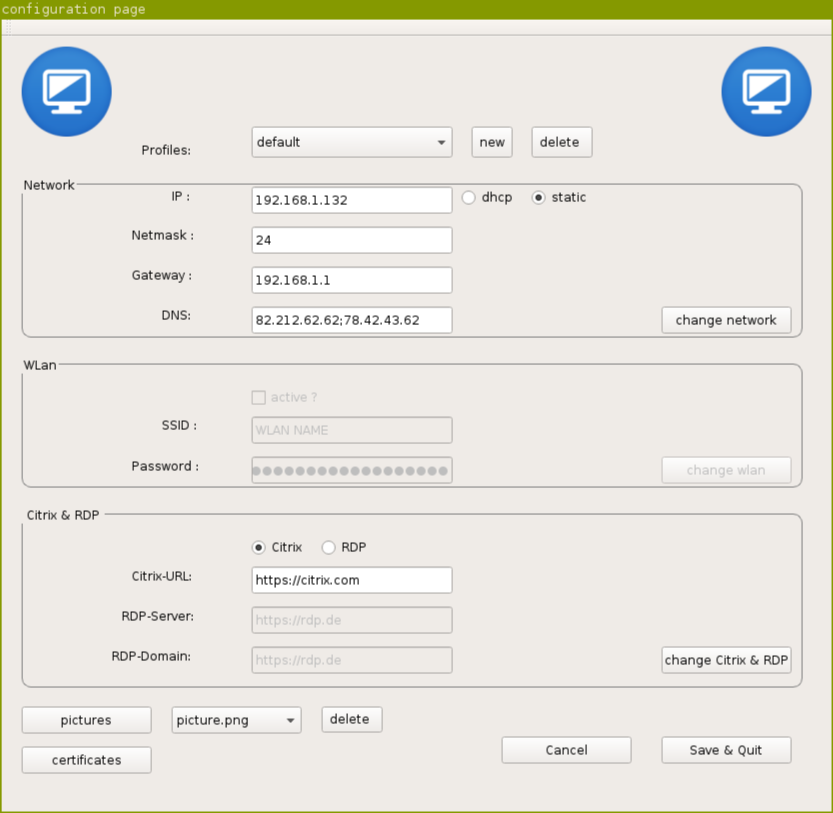
\includegraphics[scale=0.35]{ConfigPage}}}%
\begin{frame}
	\begin{flushright} 
	\tikzset{
		bend angle=45,
		pre/.style			={<-,shorten <=1pt,>=stealth',semithick},
		post/.style			={->,shorten >=1pt,>=stealth',semithick}, 
		line/.style			={-,semithick}, 
		place/.style			={rectangle,draw=blue!50,fill=blue!20,thick,inner sep=0pt,minimum size=5mm},
		double1/.style			={circle,draw=blue!50,fill=blue!0,thick,inner sep=0pt,minimum size=6mm, double circle={-2pt}{orange} },
		transition/.style		={rectangle,draw=black!50,fill=red!50,thick,inner sep=0pt,minimum size=4mm}, 
		decision/.style			={rectangle,draw=black!50,fill=black!20,thick,inner sep=0pt,minimum size=4mm}, 
		%empty/.style			={circle, text opacity=1, draw, draw=none, fill, fill=none, thick}
	}
	\begin{tikzpicture}
		\node[transition] 		(root)								{Change-Button};
		\node[decision] 		(proof)			[below=of root]				{kein System-Fehler}
			edge [pre] 					node[auto,swap]	 			{Eingaben prüfen}
			(root);	
		\node[place] 			(Fail)			[left=of proof]				{developer exception}
			edge [pre] 					node[auto]	 			{Nein}
			(proof);	
		\node[decision] 		(Edge1)			[left=of Fail]				{}
			edge [pre] 					node[auto,swap]	 			{catch}
			(Fail);	
		\node[place, double]		(log)	 		[below=of Edge1] 			{Benutzerinfo}
			%edge [post, bend left]		 	 		node[auto] 				{0,1}
			%(Start)
			edge [pre]		 	 		node[auto, swap]			{}
			(Edge1);	
		\node[place, double]		(logentry) 		[above=of Edge1] 				{Log-Eintrag}
			edge [pre]		 	 		node[auto, swap]		{}
			(Edge1);	
		\node[decision]		 	(Edge)			[below=of proof]			{Eingaben korrekt?}
			edge [pre] 					node[auto,swap]	 			{Ja}
			(proof);	
		\node[decision] 		(Start)			[below=of Edge]				{}
			edge [pre] 					node[auto,swap]	 			{}
			(Edge);	
		\node[place] 			(Wrong)			[left=of Start] 			{customer exception}
			edge [pre] 					node[auto]	 			{Nein}
			(Start);	
		\node[place] 			(Map)			[below=of Start] 			{in Map sichern}
			edge [pre] 					node[auto,swap] 			{Ja}
			(Start);	  
		\node[place, double]		(Fourth) 		[left=of Wrong] 			{Benutzerinfo}
			edge [pre]		 	 		node[auto, swap]			{catch}
			(Wrong);	
		\node[place, double]		(Quit) 			[below=of Map] 				{Eingaben prüfen $\Rightarrow$NetworkManager \& Profil aktualisieren}
			edge [pre]		 	 		node[auto, swap]			{Save \& Quit}
			(Map);	
		\node[place, double]		(Cancel) 		[left=of Map] 				{Map verwerfen}
			edge [pre]		 	 		node[auto]				{Cancel}
			(Map);	
	\end{tikzpicture}
	\end{flushright} 
\end{frame}
}


\begin{comment}
	Zum Beispiel muss eine IP-Adresse eine Form wie "192.168.1.32" haben. 

	System-Fehler = zB Datei kann nicht geöffnet werden
	Nachdem eine Exception geworfen wurde, wird natürlich der gerade ausgeführte Code unterbrochen 
\end{comment}



\subsection{Netzwerk, WLan, Citrix \& RDP}

	\begin{frame}
		\centering
		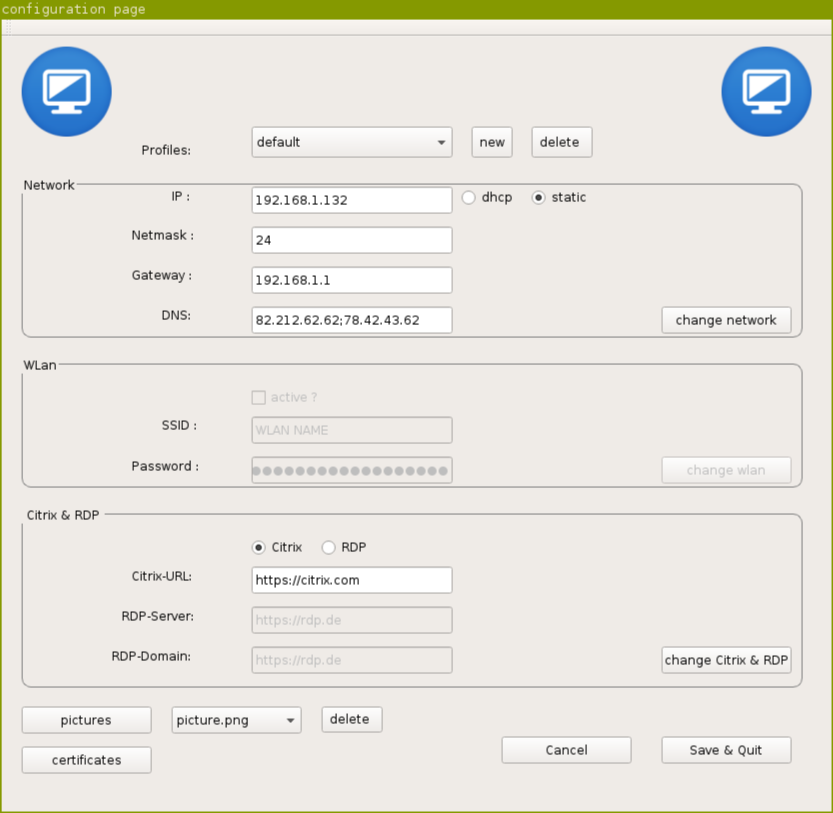
\includegraphics[scale=0.35]{ConfigPage}\\
			%\raisebox{-49mm}[5mm][5mm]{\includegraphics[scale=0.2]{../Bilder/spectrum}}
	\end{frame}

	\begin{comment}
		Citrix & RDP
		Vebindungsart: Citrix ODER RDP
		Hier können eine Citrix-URL, ein RDP-Server und eine RDP-Domäne eingegeben werden. 
		"Change Citrix & RDP": Eintrag in Verbundungstyp auf "nicht leer" bzw. keinen Whitespace überprüft
		Network & WLan

		Netzwerk
		Alle Eingabeparameter des Netzwerkes und des WLans werden werden auf ihre Sinnhaftigkeit hin überprüft. 
		Das bedeutet, dass zum Beispiel die IP dahingehend überprüft, dass sie nach dem Format 
		w.x.y.z mit w,x,y,z in [0,255] aussehen. 
		Für diese Tests wurden reguläre Ausdrücke verwendet. Ein Beispiel ist dieser: 

		REGEX
	\end{comment}


%%%%%%%%%%%%%%%%%%%%%%%%%%%%%%%
%regex
%%%%%%%%%%%%%%%%%%%%%%%%%%%%%%%
\defverbatim[colored]\regex{
\begin{lstlisting}
//ip-address must look like between 0.0.0.0 or 123.456.789.0 
std::regex pat {R"(^(\d{1,3}\.){3}\d{1,3}$)"};	
if (std::regex_match(temp, pat)) {
	//make more checks
} else {
	throw customer_error(
		std::string("The address must be of the Format: w.x.y.z with w,x,y,z in [0,255]")
	);
}
\end{lstlisting}
}
	\begin{frame}
		\begin{center}
			\begin{columns}
				\begin{column}{.05\linewidth}
				\end{column}
				\begin{column}{.85\linewidth}
					\regex
					\centering
					Pattern-Missmatch\\
					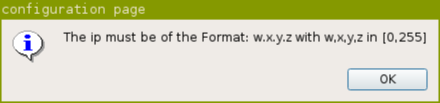
\includegraphics[scale=0.60]{regex_fail}\\
				\end{column}
			\end{columns}
		\end{center} 
	\end{frame}





	\begin{frame}
		\centering
		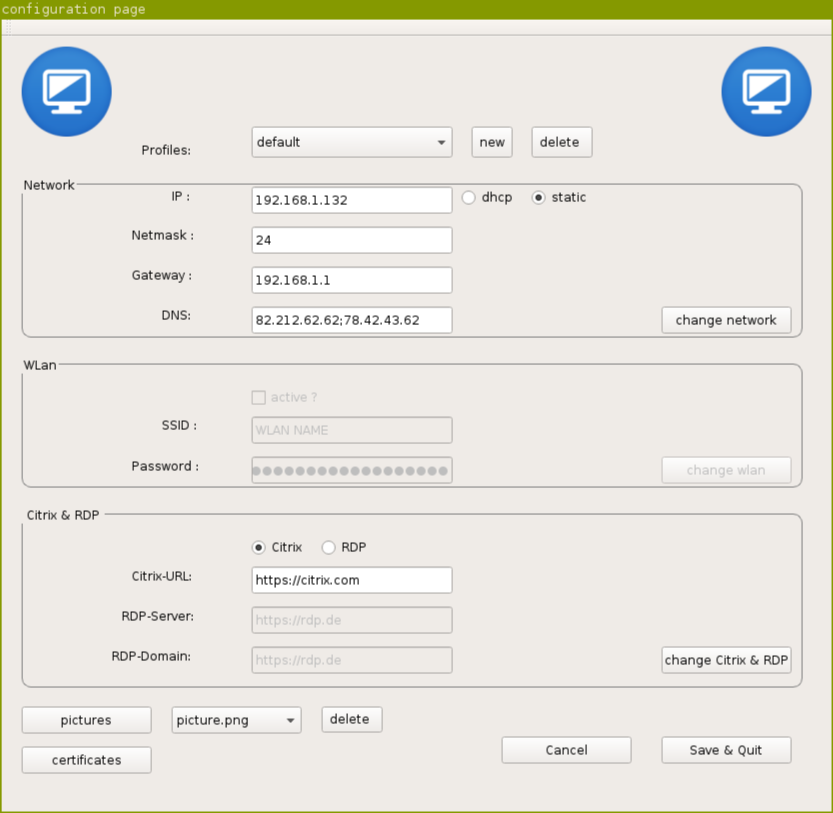
\includegraphics[scale=0.35]{ConfigPage}\\
			%\raisebox{-49mm}[5mm][5mm]{\includegraphics[scale=0.2]{../Bilder/spectrum}}
	\end{frame}





\begin{comment}
  Gateway, DNS und Netmask werden wie die IP überprüft, wobei bei der Netmask zustätzlich gilt, dass diese 
    wenn w < 255 => x = 0 gelten muss, usw. 

  Die Netmask kann im auch in einem Format von x in [0,32] angegeben werden.
    Abschließend wird überprüft, ob die IP bezüglich der Netmask mit dem Gateway übereinstimmt, dass heißt, an Stellen, 
    an denen die Netmask 255 ist, müssen IP und Gateway übereinstimmen. 


  - WLan: 
    keine MAC-Adresse: WLan deaktiviert. 
    Passwort auf Länge überprüfen.  min. 8 & max. 63 Zeichen 
    Darüber hinaus darf kein "'" (einfaches Aphostroph) im Passwort enthalten sein, ansonsten kann es zusammen mit der SSID des WLans 
    über wpa_passphrase nicht verschlüsselt werden. 

  - NetworkManager:
    "Save & Quit"-Button geklickt:
    Profil-Map: 1 Datei für Ethernet & 1 Datei für WLan, falls aktiv
    Datei-Besitzer & Gruppe: root 
    Nur Besitzer: lesen & schreiben 
    Werden diese Anforderungen nicht erfüllt, so erkennt der NetworkManager diese Dateien nicht. 
    Neustart NetworkManager 


  - Kommandozeilenbefehle:  
    Befehle wie: nm-Neustart oder Erhalten der MAC-Adresse, Kommandozeilenbefehle ausführen & auslesen
    "popen" zusammen mit "pclose"
    Bei Exception: keine offene Pipe zurückbleibt =>unique_ptr mit zustätzlichem Destruktorbefehl
\end{comment}

%%%%%%%%%%%%%%%%%%%%%%%%%%%%%%%
%unique_ptr
%%%%%%%%%%%%%%%%%%%%%%%%%%%%%%%
\defverbatim[colored]\uniqueptr{
\begin{lstlisting}
// unique_ptr with custom deleter function for FILE*: pclose().
//EXPLANATION
unique_ptr<FILE,   			//raw pointer type: FILE*
int(*)(FILE*)> 		        //type: pclose() prototype
myFile(popen("myfile","r"), //(FILE*) is returned by popen()
pclose );              	    //deleter function: pclose()

//USEAGE:
unique_ptr <FILE, int(*) (FILE *)> file(popen(cmd,"r"), pclose);
output = read_out_stream(move(file));

//function prototype using this pointer
string read_out_stream(unique_ptr <FILE, int (*)(FILE *)> fp)
\end{lstlisting}
}
	\begin{frame}
		\begin{center}
			\begin{columns}
				\begin{column}{.05\linewidth}
				\end{column}
				\begin{column}{.85\linewidth}
					Ausführen von Konsolenbefehlen:\\
					\uniqueptr
				\end{column}
			\end{columns}
		\end{center} 
	\end{frame}


\begin{comment}
	Test
	Zusätzlich einzelne Funktionen mit Unit-Test von Qt (QTest) auf Korrektheit überprüfen. 
	Seit Qt 5.3 kann auch eine Exception ein korrekter Rückgabewert sein. 
	Erweiterung der Tests geplant. 
\end{comment}

\section{Ausblick}
%for distance between some items 
\makeatletter
\newcommand{\setlistspacing}[2]{\def\@ld{#1}\expandafter\def\csname
@list\romannumeral\@ld \endcsname{\leftmargin\csname
leftmargin\romannumeral\@ld \endcsname
              \topsep    #2
              \parsep    0\p@   \@plus\p@
              \itemsep   #2}}
\makeatother
%{\setlistspacing{2}{2ex} %not in use right now
\begin{frame}
\Large
\begin{itemize}
	\item Einstellung der systemweiten Sprache und des Tastaturlayouts
	\item Menü zur Sprache-Konfiguration
	\item Datenbank zur Profile-Speicherung
\end{itemize}
	
\end{frame}
%}

\normalsize

\section{Live-Demo}



%%%%%%%%%%%%%%%%%%%%%%%%%%%%%%%%%%%%%%%%%%
% bis hier hin alles bearbeitet
%%%%%%%%%%%%%%%%%%%%%%%%%%%%%%%%%%%%%%%%%%

\begin{comment}
Live Demo:
IP und Netmask, aber Gateway abweichend.

WLan Passwort verschlüsseln lassen. 

static und dhcp
\end{comment}


%End
\section*{ }
\begin{frame}
\frametitle{Dankeschön}
\centering
Weitere Informationen sind im Wiki enthalten\\

\{R"(Bitte [(?stellen Sie)|(?stell)]\{1\} offene Fragen nach der Live-Demo)?"\}
%\begin{figure}
	%\begin{wrapfigure}[14]{c}{6.2cm}
	% \includegraphics[scale=0.2]{tree}
	%\end{wrapfigure}
%\end{figure}

\end{frame}

\end{document}
